%% josis.tex 1.2   2009-06-11    JoSIS latex template
%------------------------------------------------------------------
% Filename: josis.tex
%
% This file is intended as a template for typesetting articles for the
%
%                        Journal of Spatial Information Science.
%
% Please edit this template to generate your own formatted manuscripts
% for submission to JOSIS. See http://josis.org for further details.
%
% The template was developed by Matt Duckham (http://www.duckham.org)
%

% Required documentclass definition for JOSIS
\documentclass{josis}
\usepackage{graphics}
\usepackage{subfigure}
\usepackage[colorlinks=true,urlcolor=blue]{hyperref}
\usepackage{enumerate}

% Link as footnote
\newcommand{\furl}[1]{    $\,$\footnote{$\,$\url{#1}}}

% Article details for accepted manuscripts will be added by editorial staff
%\josisdetails{%
%   volume=0, number=0, year=2009, firstpage=0, lastpage=1,
%   received={January 1, 2009},
%   revised={March 1, 2009},
%   accepted={May 1, 2009},
%   published={June 1, 2009}
%}


% Add the running author and running title information
\runningauthor{\begin{minipage}{.9\textwidth}\centering Michel, Grizonnet, Jaen, Hermitte, Guinet, Harasse, Malik, Savinaud\end{minipage}}
\runningtitle{Large-scale segmentation of VHR satellite images using Orfeo ToolBox}

% Document begins
\begin{document}

% Insert your own title
\title{Large-scale segmentation of Very High Resolution satellite images using Orfeo ToolBox}

% Insert your manuscipts authors, affiliations, and addresses
\author{Julien Michel}
\author{Manuel Grizonnet}\affil{CNES, DCT/SI/AP, BPI 1219 18, avenue Edouard Belin, 31401 Toulouse Cedex 09 - France}
\author{Arnaud Jaen}
\author{Luc Hermitte}
\author{Jonathan Guinet}
\author{S\'ebastien Harasse}
\author{Julien Malik}
\author{Micka\"el Savinaud}
\author{Guillaume Pasero}\affil{CS Syst\`emes d'Information, Division ESPACE \& Renseignement - D\'epartement APPLICATIONS, Parc de la Grande Plaine - 5, Rue Brindejonc des Moulinais - BP 15872, 31506 Toulouse Cedex 05 - FRANCE}


\maketitle

% Add 5-10 keywords for every submission
\keywords{Open-source software, segmentation, remote sensing images, GIS}

% Add a short abstract of 150-250 words
\begin{abstract}
TO COMPLETE
Segmenting objects across a very high resolution scene and with a controlled
quality is a difficult task for which no method has reached a sufficient level
of performance to be considered as operational.

Even if we leave aside the question of segmentation quality and consider that we
have a method performing reasonably well on our data and objects of interest,
the task of scaling up segmentation to real very high resolution data is itself
challenging. First, we can not load the whole data into memory, and there is a
need for on the flow processing which does not cope well with traditional
segmentation algorithms. Second, the result of the segmentation process itself
is difficult to represent and manipulate efficiently.

The experience of segmenting large remote sensing images is packed into a single
segmentation in the ORFEO ToolBox library. This application provide a complete
framework to get a vector segmentation output that can be used in GIS software
but it is only a first step toward providing an open source large scale Object
Based Image Analysis (OBIA) and spatial reasoning framework.

\end{abstract}


% Your main text begins here.
\section{Introduction}

With the increase of the spatial resolution of satellite images,
analysis techniques such as Object Based Image Analysis (OBIA) or Spatial
Reasoning \cite{inglada2009qualitative} have become widely studied and
used. Because they use objects rather than pixels as their primitives,
these methods are very well adapted to represent and extract the
information contained in very high resolution imagery (VHR). Moreover,
reasoning on objects is often supported by very sound theories. Yet
one of their severe weakness is the process of obtaining the objects
themselves: segmentation is widely used as a pre-processing step for
these techniques, and it is well known that the task of segmenting all
categories of object of interest, across a large very high resolution
scene and with a controlled quality is a difficult task for which no
method has reached a sufficient level of performance to be considered
as operational.

Even if we leave aside the question of segmentation quality and
consider that we have a method performing reasonably well on our data
and objects of interest, the task of scaling up segmentation to real
very high resolution data is itself challenging. First, we can not
load the whole data into memory, and there is a need for on the flow
processing which does not cope well with traditional segmentation
algorithms \cite{shi2000normalized}. Second, the result of the
segmentation process itself is difficult to represent and manipulate
efficiently.

There are, to our best knowledge, few open source software able to
overcome these issues. In the frame of the development of the Orfeo
ToolBox \cite{}, we therefore initiated some work to provide software
components for this purpose.

\section{About the Orfeo ToolBox}

The Orfeo Toolbox (OTB) is an open-source (CeCILL license), remote sensing-oriented, image processing library. Initiated by the French Space Agency (CNES) in the frame of the ORFEO accompaniment program~\furl{http://smsc.cnes.fr/PLEIADES/A_prog_accomp.htm}. Based on the medical image processing library Insight ToolKit (ITK), the OTB provides to its users an extensive set of algorithms and functionalities dedicated to remote sensing data exploitation. More specifically, the OTB embeds efficient approaches to handle large data using advanced streaming and multi-threading strategies. Thus, OTB-based processing chains take advantages of both optimized Input/Output access and streamed/multi-threaded filtering to perform efficient processing.

OTB is based on a large set of open-source libraries which contribute to expand the OTB ecosystem. The main part of this ecosystem are described in the figure~\ref{fig:ecosystem}. Through the use of these libraries, OTB offers the possibility to manipulate and process the main remote-sensing data from optical to hyperspectral through SAR sensor. The processing capabilities of OTB library covers a large set of uses cases from optical calibration and data projection to image segmentation and classification. An exhaustive list can be found in the documentation.

\begin{figure}[!htb]
\centering
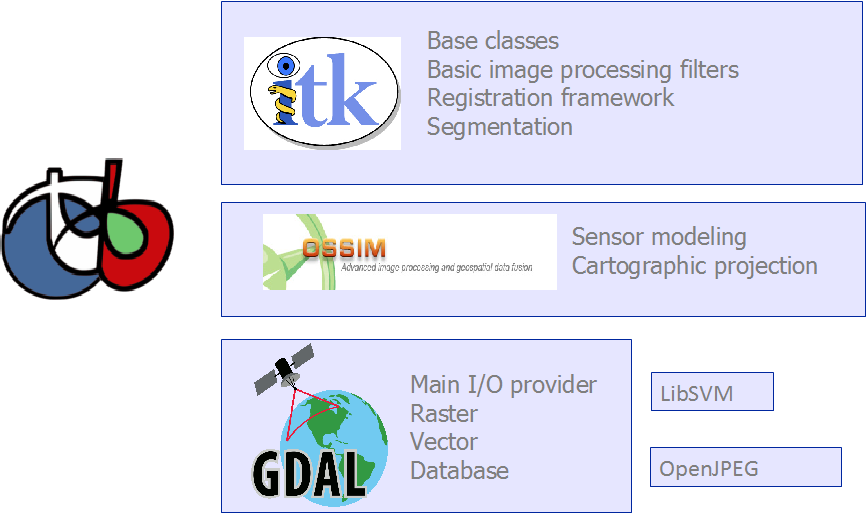
\includegraphics[width=0.8\textwidth]{Pictures/otb_ecosystem}\label{fig:ecosystem}
\caption{Orfeo ToolBox ecosystem}
\end{figure}

The main way to access to the OTB capabilities for end-users is to use the set of applications offered by OTB. The OTB Applications have been recently improved to answer to the increasing need to interface OTB capabilities into other software and to provide a better access to end-users. These OTB applications are designed to be more user-friendly and to be auto-loaded into appropriate tools without recompiling (as a shared library). Currently Orfeo ToolBox ships the following tools:
\begin{itemize}
\item A command-line launcher and a set of command-line tools
\item A graphical launcher and a set of tools based on a QT interface which provide ergonomic parameters setting, display of documentation, and progress reporting,
\item A SWIG interface, which allows to use any application into a high-level language such as Python or Java for instance.
\end{itemize}
Moreover, through the Sextante project, OTB applications are also available into the QGIS project. QGIS users have now an easy way to process their data and combine OTB processing with other tools.

To follow the best practices of an open-source project, OTB offers via a public official repository a high quality code to promote dissemination and contribution. Thus, the library is built and tested on a nightly basis. The results are available publicly which ensures multi-platform consistency and continuous validation. Moreover, OTB encourages full access to the details of all the algorithms through extensive documentation. This documentation is divided between class documentations, the software guide and a cookbook with use cases~\furl{http://orfeo-toolbox.org/otb/documentation.html}.

\section{Segmenting very large images with Orfeo ToolBox}


\subsection{Representations and data structures for segmentation results}

In this section, we review three standard structures to store
segmentation results, and explain why we selected the third one for
our framework.

The most common way of representing segmentation results from an image
processing perspective is to derive a raster where each pixel contains
the unique label of the segment it belongs to. Such a raster is also
known as label image. Yet this representation has numerous
drawbacks. First, accessing all pixels of a given segment identified
by its label requires parsing the whole label image. Second, storing
large segmentation results with billions of segments might require a
high number of bits to represent the label, thus increasing
dramatically the size of the output. Last, the constraint of label
uniqueness is very strong, yet not very useful: it is required since
label images only provides an implicit description of segments, based
on neighboring pixels with same labels. This representation is of
limited interest for our purpose.

A second representation of segmented image which is further from image
processing is the map of label objects \cite{lehmann2008label}. A segment is
represented in Run Length Encoding (RLE), and all segments are indexed
by a unique label in a map. The RLE representation is more compact,
the map allows fast access to a segment given its label, and it also
allows to store attributes related to a segment, which is a first step
toward Object Based Image Analysis. The main drawback of this
representation is that there are no standard file format able to store
it on a file system, and it requires to convert either to or from
raster or vector representation at each read or write
operation. Moreover, this representation is neither really raster nor
really vector. Therefore, operations like walking pixels in the
segment or following its contour are more complex.

Neither of these two structures can fit our needs: the first one is
highly inefficient, while the second one lacks of existing file
formats. We chose to store our segmentation results as boundaries in a
vector structure and file format. This has numerous advantages. First,
it overcomes the issue of scaling up to large image segmentation: a
collection of vector objects, i.e. polygons or multi-polygons, is a
compact representation which will grow linearly with the size of the
image, and does not need an explicit unique indexing label. Second,
there are several file formats and even databases to represent this
kind of vector data, especially in the GIS world. Last, using such
formats guarantees a full interoperability between the segmentation
tools and most GIS software, which is desirable.

As described in the next section, we intend to derive a generic
framework for large scale remote sensing images segmentation, thus we
need to be compatible with the raster output of most segmentation
algorithms, which usually produce a label image. For this purpose, we
need a component for exact conversion between the raster
representation and the vector one. We take advantage of the
polygonization and rasterization algorithms provided by GDAL
\cite{}. To handle on the flow input and output to vector data files
and databases, we then use the full extent of OGR functions
\cite{}. This abstraction layer allows our tool to address
simple file formats like ESRI Shapefile or complex databases like
PostGIS seamlessly.

\subsection{Segmentation algorithms}

\begin{figure}[!htbp]
\centering
\subfigure[Connected Components (optimal LUT)]{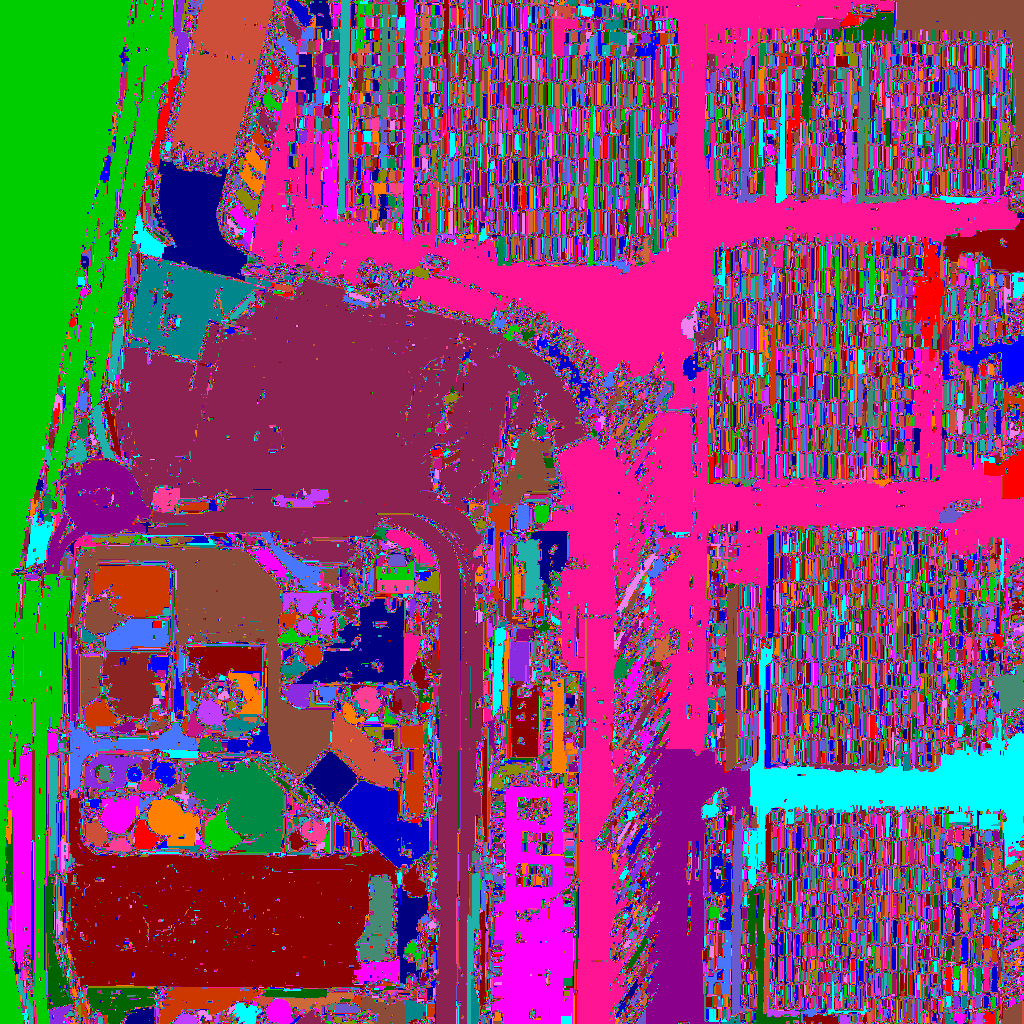
\includegraphics[width=0.26\textwidth]{Pictures/second_cc_color_optimal}\label{fig:cc_optimal}}
\qquad
\subfigure[Connected Components (natural LUT)]{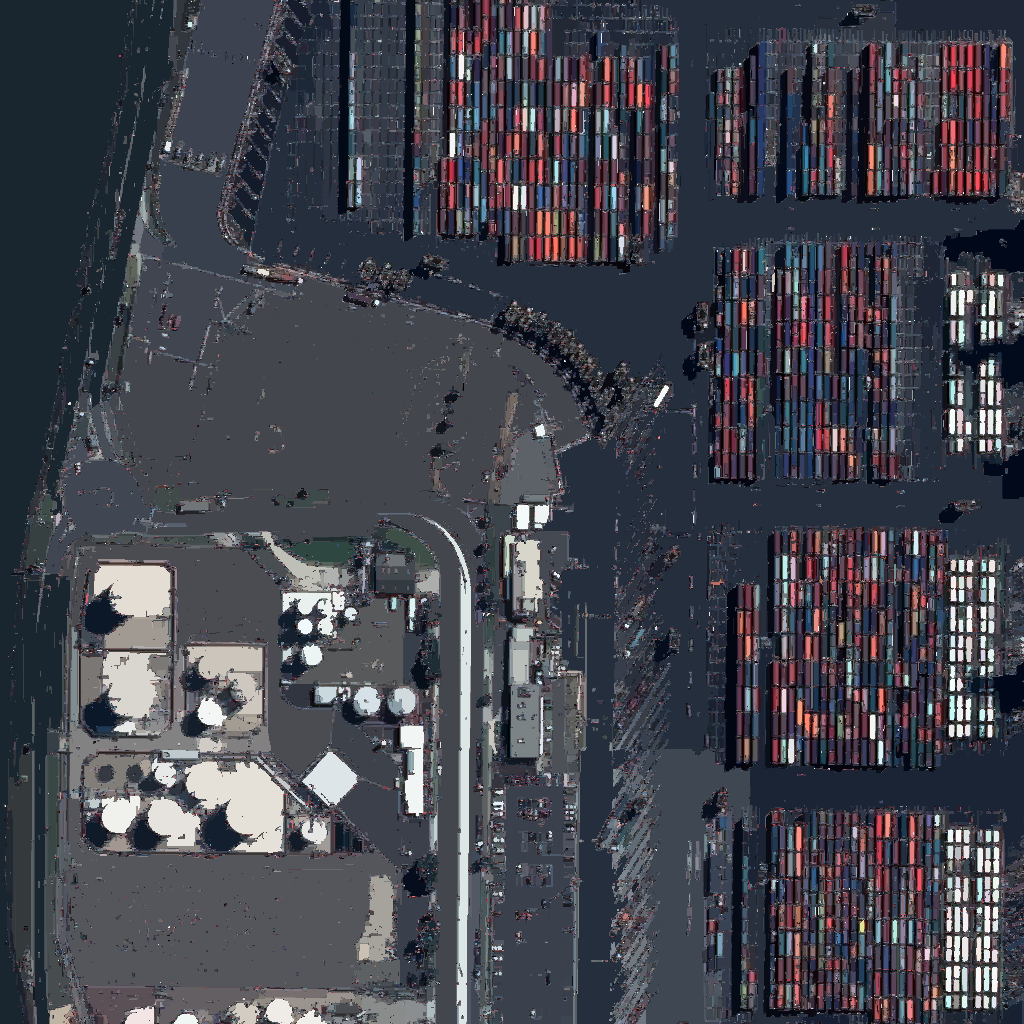
\includegraphics[width=0.26\textwidth]{Pictures/second_cc_color_image}\label{fig:cc_natural}}\\

\subfigure[Watershed (optimal LUT)]{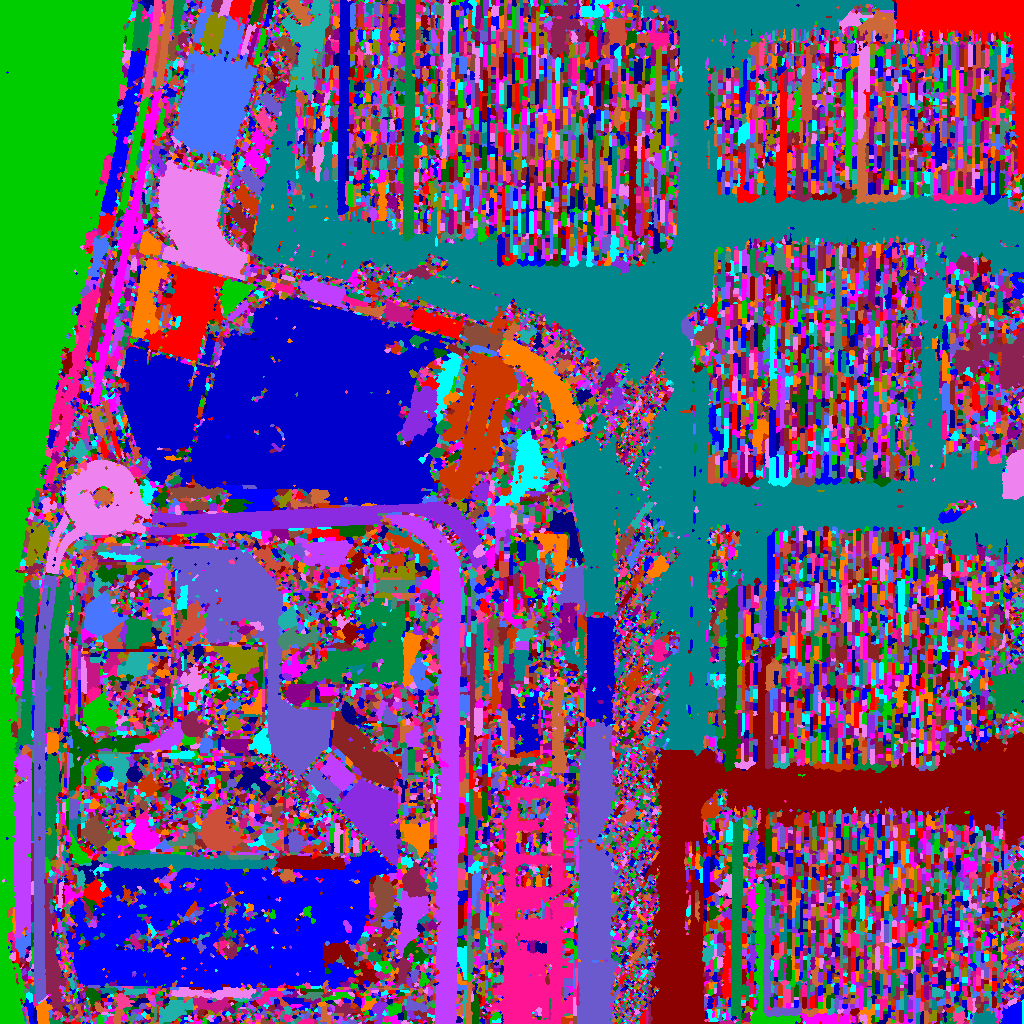
\includegraphics[width=0.26\textwidth]{Pictures/watershed_color_optimal}\label{fig:ws_optimal}}
\qquad
\subfigure[Watershed (natural LUT)]{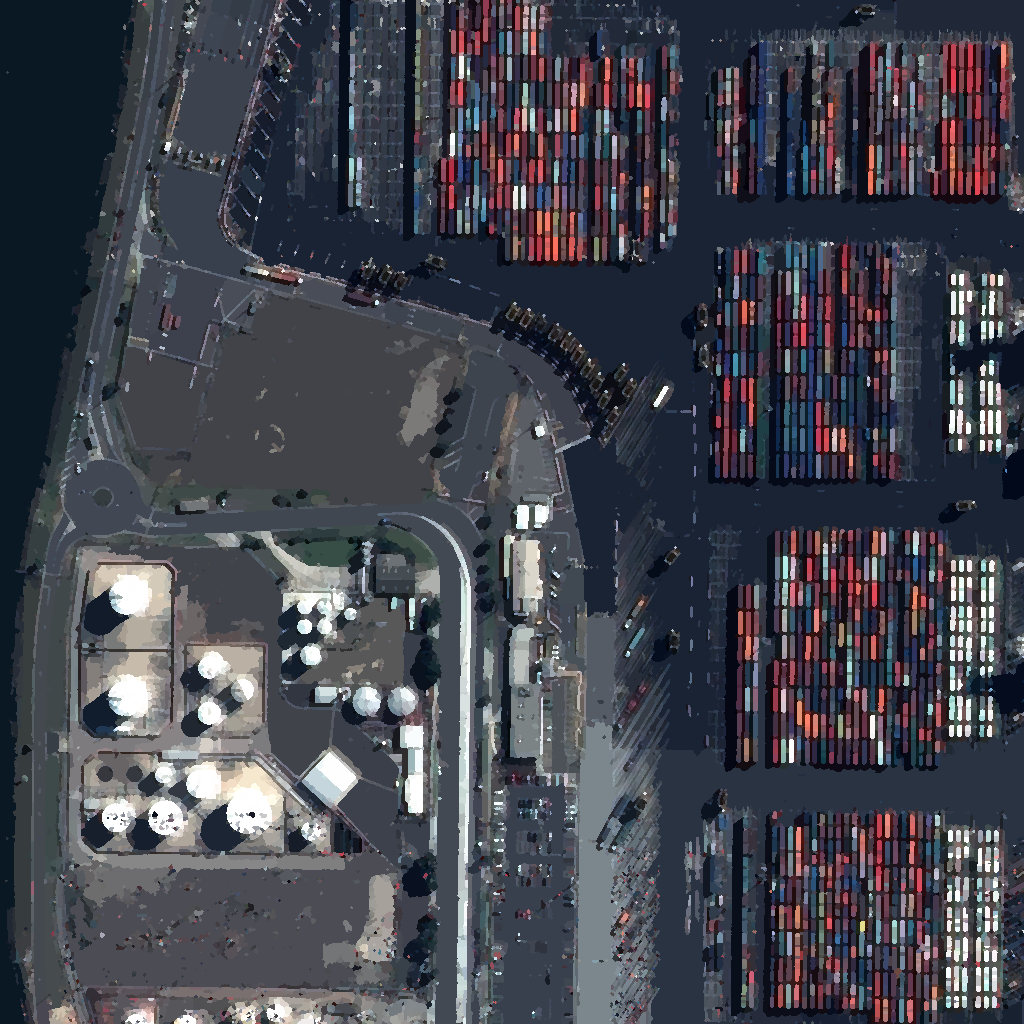
\includegraphics[width=0.26\textwidth]{Pictures/watershed_color_image}\label{fig:ws_natural}}\\

\subfigure[Mean-Shift (optimal LUT)]{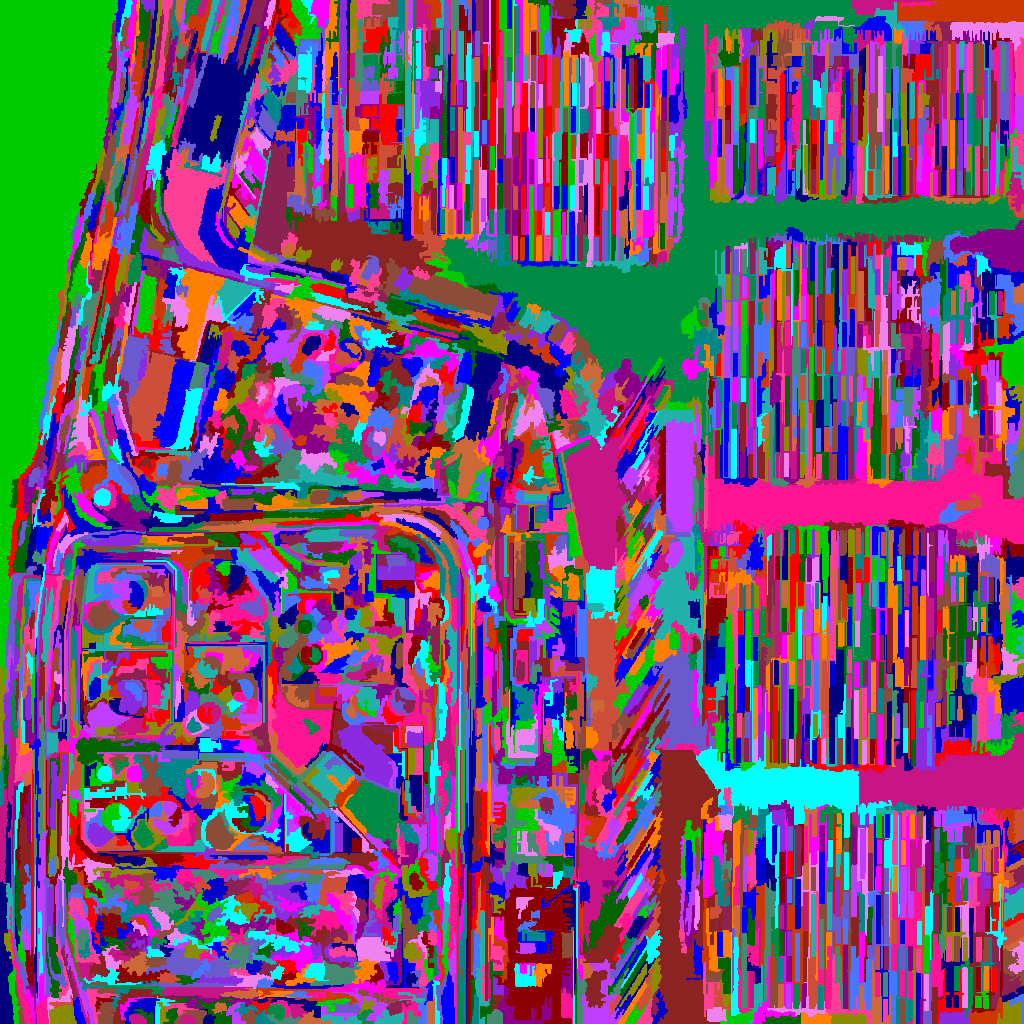
\includegraphics[width=0.26\textwidth]{Pictures/meanshift_color_optimal}\label{fig:ms_optimal}}
\qquad
\subfigure[Mean-Shift (natural LUT)]{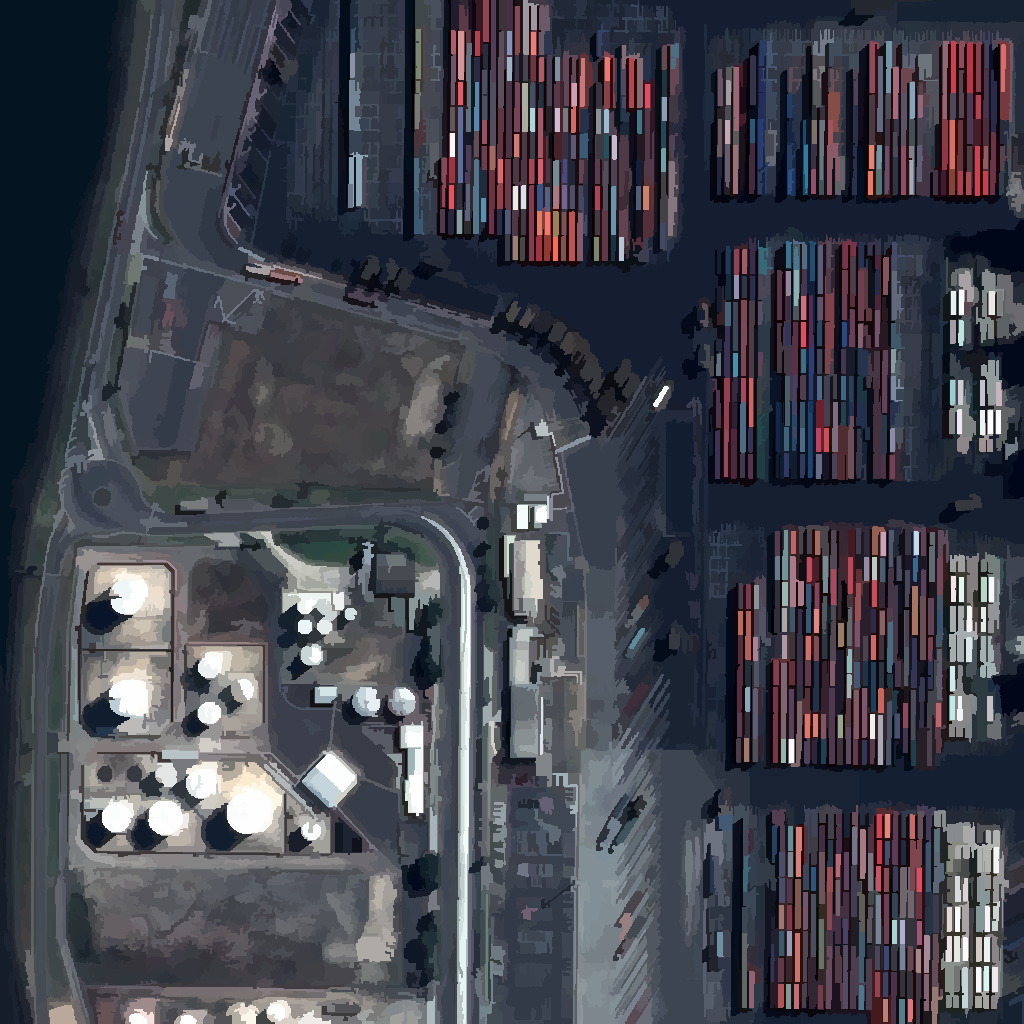
\includegraphics[width=0.26\textwidth]{Pictures/meanshift_color_image}\label{fig:ms_natural}}\\
\subfigure[Morphological Profiles (optimal LUT)]{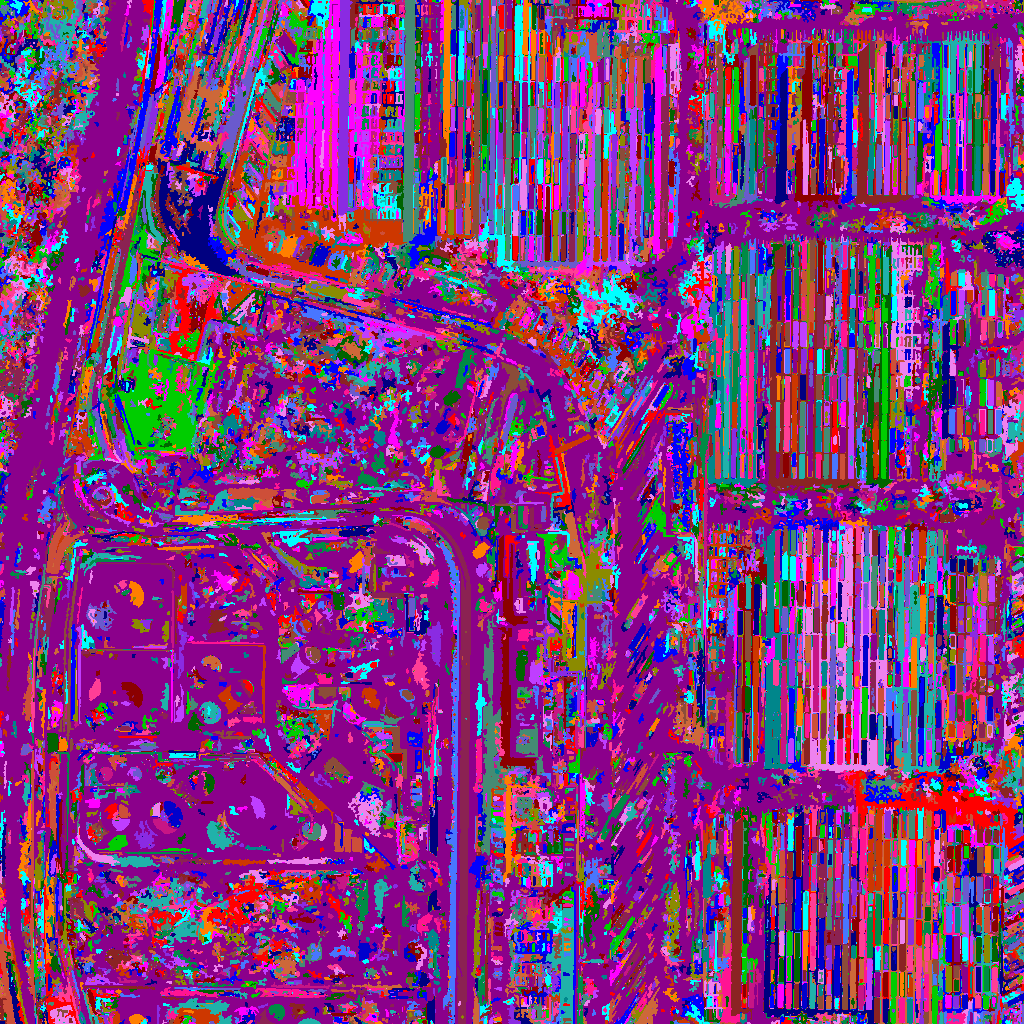
\includegraphics[width=0.26\textwidth]{Pictures/geomorpho_color_optimal}\label{fig:gm_optimal}}
\qquad
\subfigure[Morphological Profiles (natural LUT)]{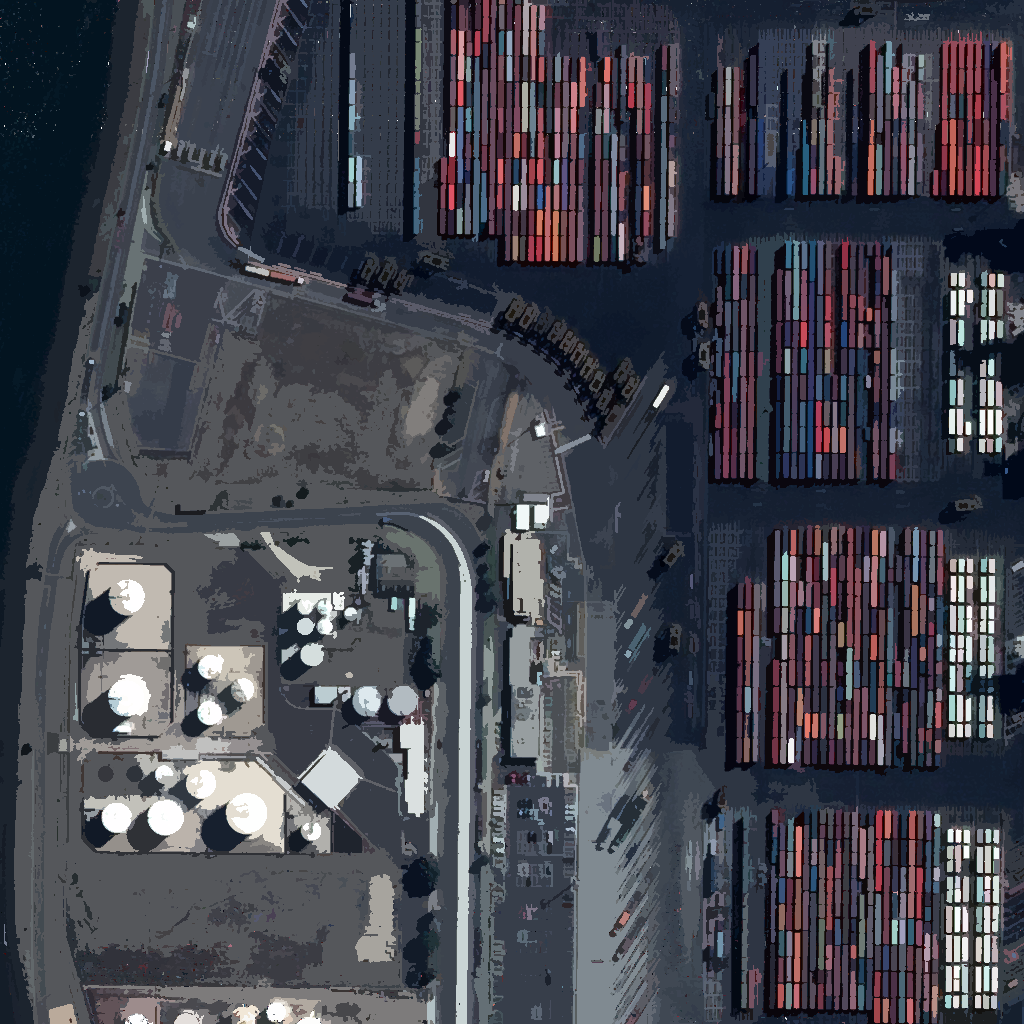
\includegraphics[width=0.26\textwidth]{Pictures/geomorpho_color_image}\label{fig:gm_natural}}
\caption{Results of various segmentation algorithms from Orfeo ToolBox}
\end{figure}


\subsection{Framework for large scale segmentation}

This section describes the generic framework that has been implemented
to support various segmentation algorithms. In the Orfeo ToolBox, 
we define a segmentation algorithm as a filter
that accepts a remote sensing image as input and produces a label
image as output. This filter is not supposed to have streaming (on the
flow) capabilities, it is allowed to require the whole input image to
produce its output. The streaming will be handled by the framework. The
filter can however make an internal use of multi-threading.
Such an algorithm shall be supported by our framework in order to
segment quite large images. For instance a basic Pleiades image
\cite{} has an extent of 40 000 by 40 000 pixels, which corresponds to
a memory size of 3.2GB assuming a single-band image with 16 bits per pixel.
Our framework works as follows:
\begin{enumerate}[1 - ]
\item Derive a tiling scheme, which depends on the following parameters:
\begin{itemize}
\item the amount of memory available on the computer
\item the file format of the input image (in some formats,
the image is already stored in tiles)
\item the user preferences
\end{itemize}
\item For each tile of the tiling scheme:
\begin{enumerate}[a - ]
\item Load the corresponding image part into memory
\item Segment the image extract with the segmentation algorithm
\item Polygonize the result using a filter based on GDAL capabilities,
\item Dump the polygons to file system or database through OGR
      abstraction.
\end{enumerate}
\end{enumerate}

It is important to note that some tiling schemes are not suited for this
framework. For instance, if the image is streamed line by line, performing
a segmentation on each line independently is irrelevant.

\begin{figure}[!htb]
\centering
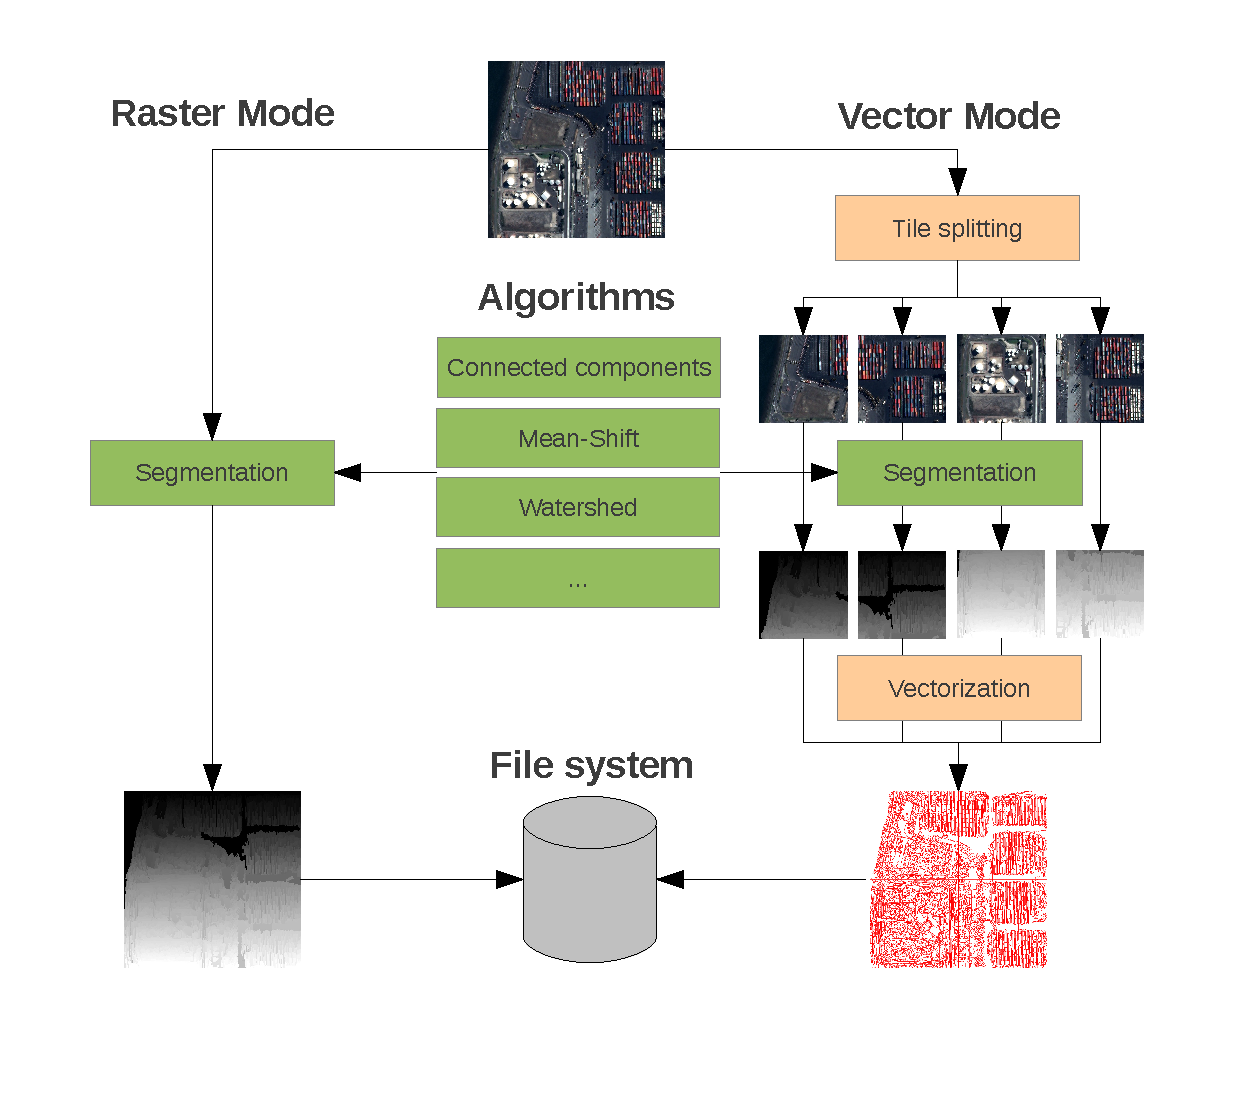
\includegraphics[width=0.8\textwidth]{Pictures/schema_ogrs}\label{fig:overview}
\caption{Overview of the large scale segmentation framework in the Orfeo ToolBox}
\end{figure}

The strength of this framework is that it will naturally scale up:
larger images will take more time to process and more space on file
system to store, but the system will never run out of the most limited
resource on most hardware, which is memory. The input image will still be
loaded tile by tile, and the polygons will be stored after each tile is
segmented. The most time consuming
operation is the segmentation, and this is where we allow for parallel
processing depending on the segmentation algorithm implementation. In the 
OTB, the typical way to perform parallel processing is to sub-divide the 
streaming tiles into smaller tiles, processed by different threads. For
instance, we implemented a multi-threaded version of the Mean Shift
algorithm \cite{Comaniciu2002mean}. This version provides a significant 
performance gain when the system has multiple processor cores.

An other key feature is that we make few assumptions on the segmentation
algorithm, and that our framework will be able to perform with any
segmentation algorithm implemented under these assumptions. The
different algorithms don't need to share the same set of parameters. They
can have their specific methods and attributes (the segmentation algorithm
can be accessed from outside the framework). The same
code already runs with a basic connected components algorithm, two
different implementations of the Mean Shift algorithm, and a Watershed algorithm.

Of course, this framework has the same drawbacks as other streaming
methods. Algorithms using global information in the input image will
produce different results depending on the tiling scheme, but this is
a lesser issue for segmentation algorithms that focus on local information.
The main drawback is over-segmentation : the regions lying on tiles borders
will be artificially split by the tiling scheme. This can be a real concern
when a big object that crosses several tiles must be segmented as one region.
We address these issues in the following section.

\begin{figure}[!htb]
\centering
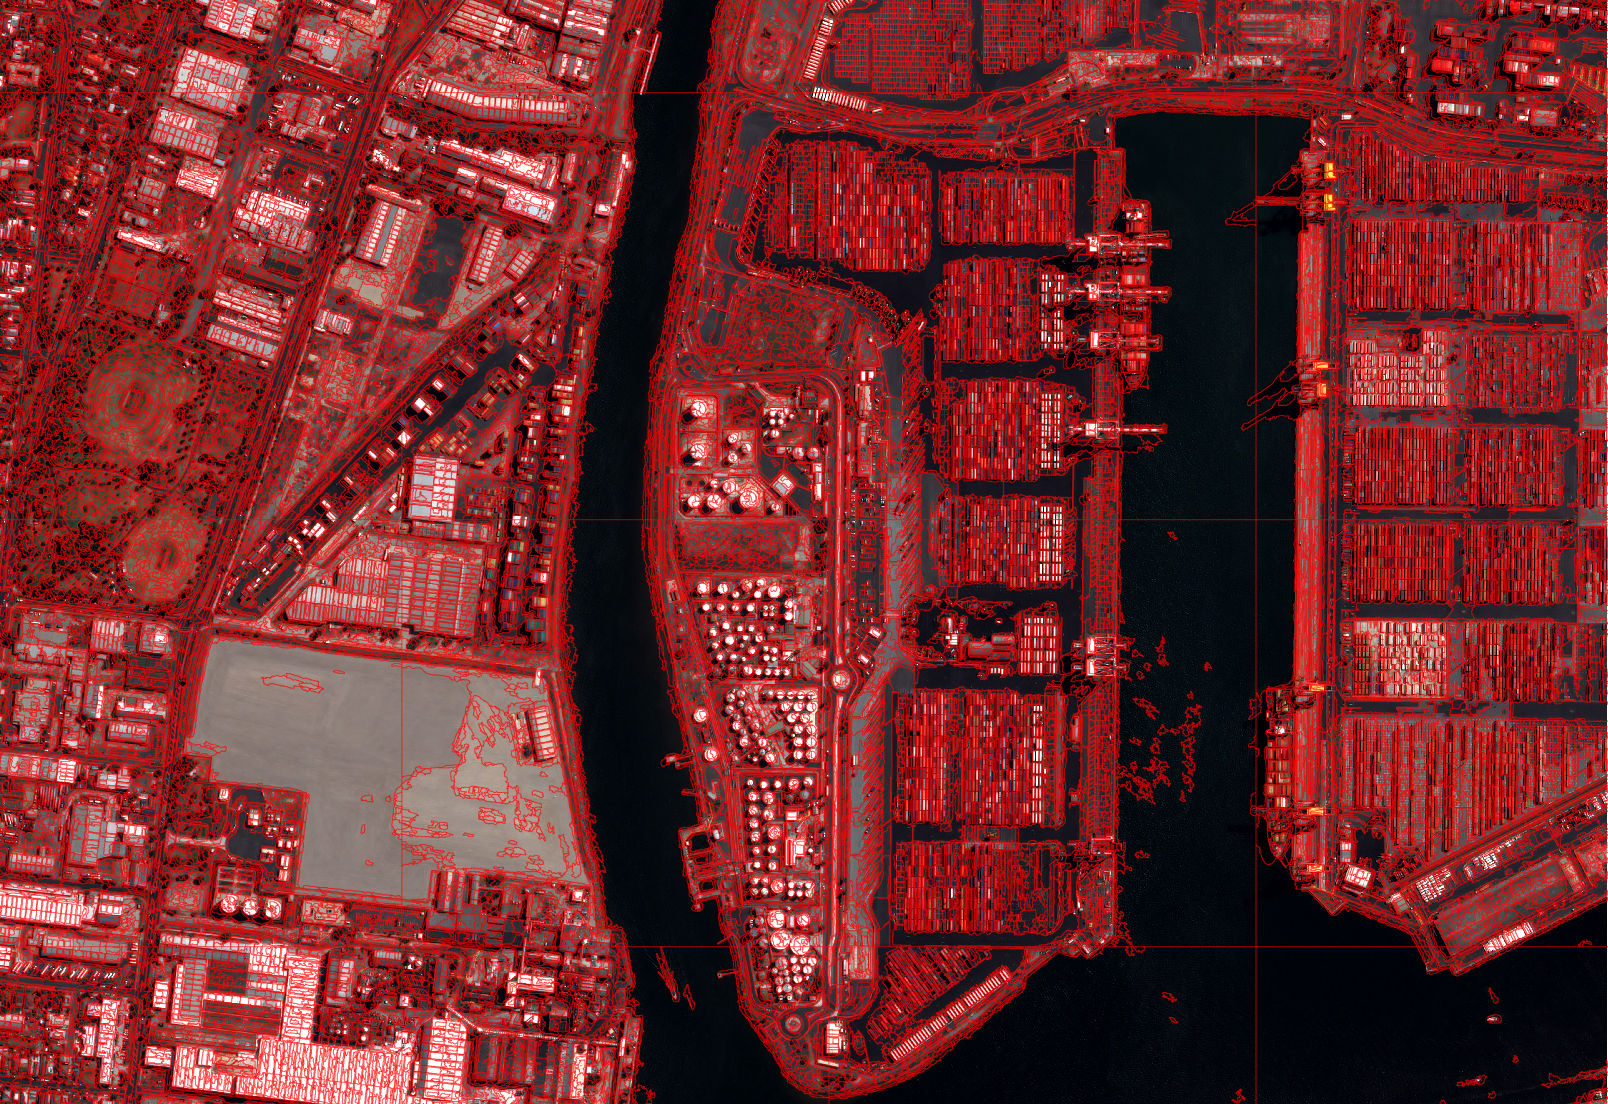
\includegraphics[width=0.9\textwidth]{Pictures/ogrs_nostitch.png}\label{fig:nostitch}
\caption{Example of large scale segmentation result displayed in QGIS}
\end{figure}


\subsection{Pre and post-processing to enhance usability}

In order to get useful results from this large scale segmentation, we
need to address several issues. The first one issue is the splitting
of the regions on the border of tiles. The naive solution we
implemented is a simple stitching rule: we post-process the vector
data by looking for neighbor polygons lying on each side of a tile
border and merge them if their contact surface is large enough. More
sophisticated techniques might be derived in the future.

\begin{figure}[!htb]
\centering
\subfigure[Stitching overview]{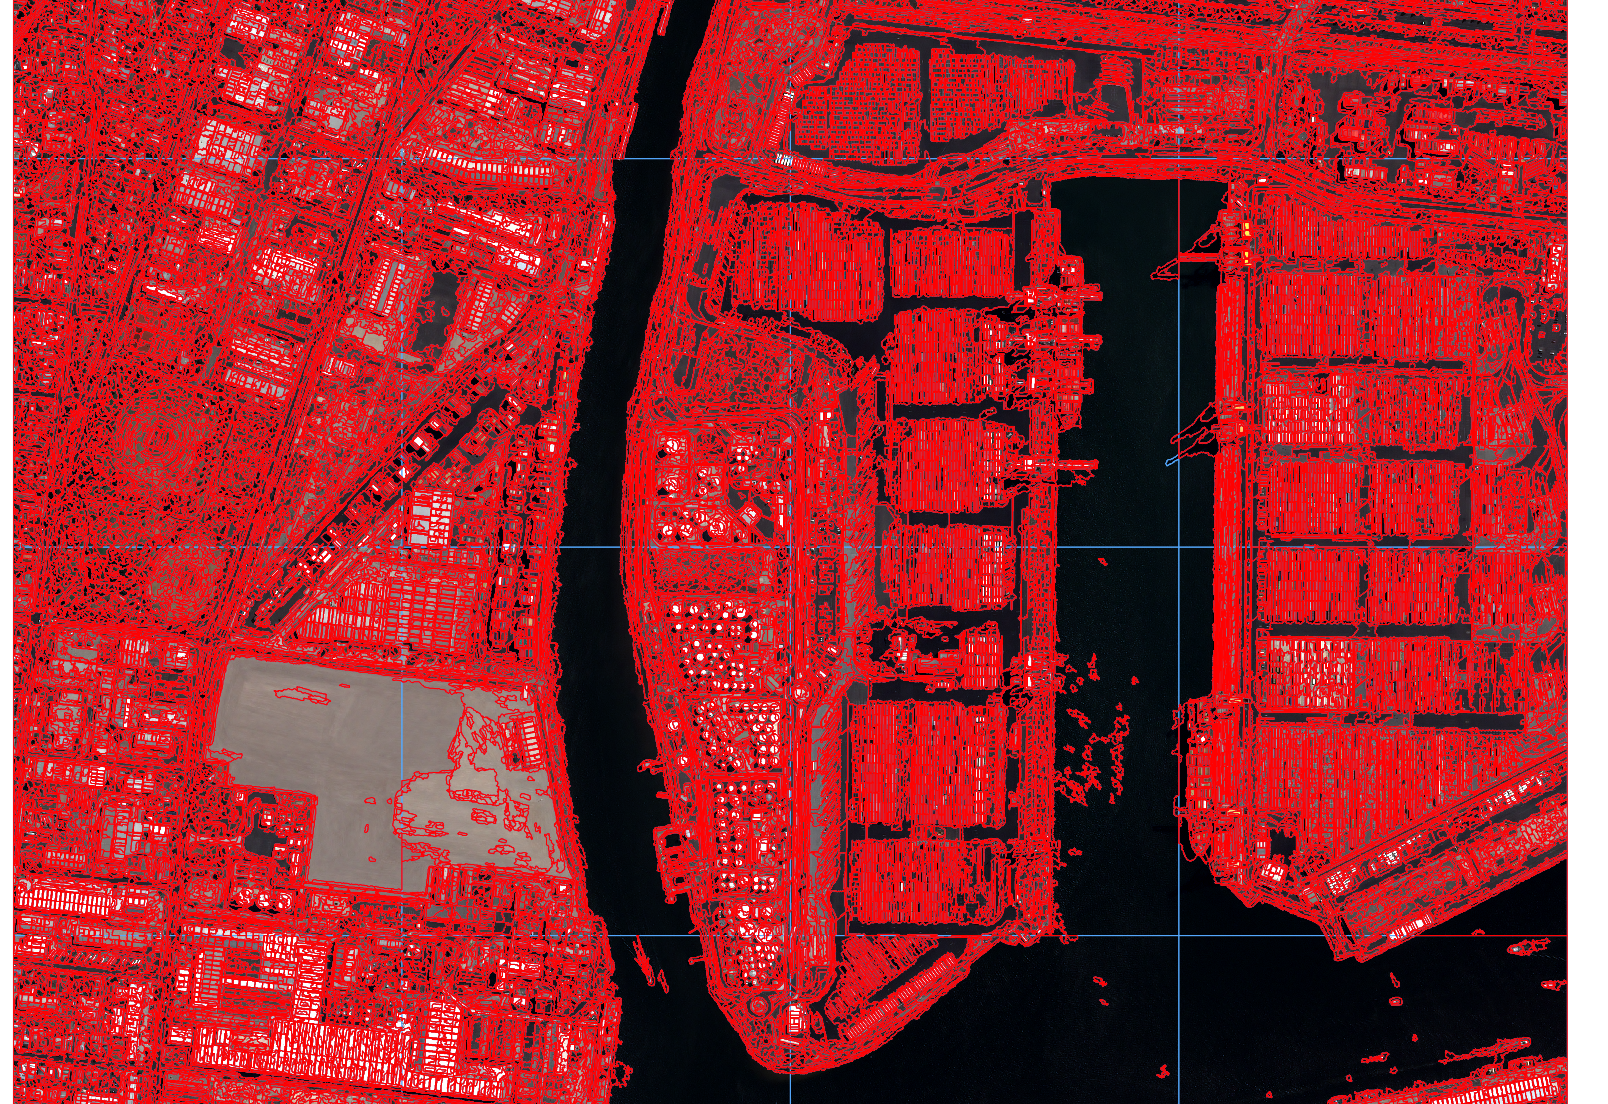
\includegraphics[width=0.9\textwidth]{Pictures/ogrs_stitch.png}\label{fig:stitch}}\\
\subfigure[Stitching off (detail)]{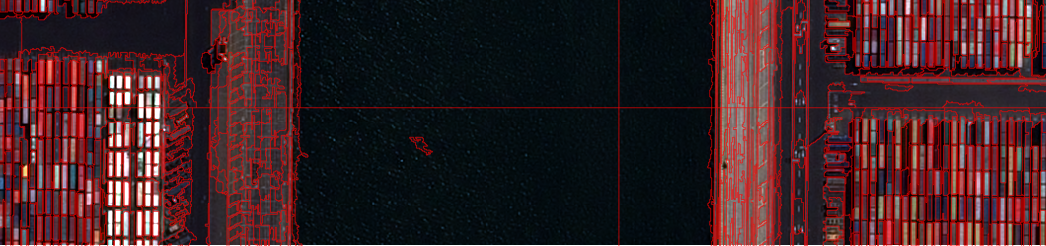
\includegraphics[width=0.45\textwidth]{Pictures/ogrs_nostitch_xt.png}}
\subfigure[Stitching on (detail)]{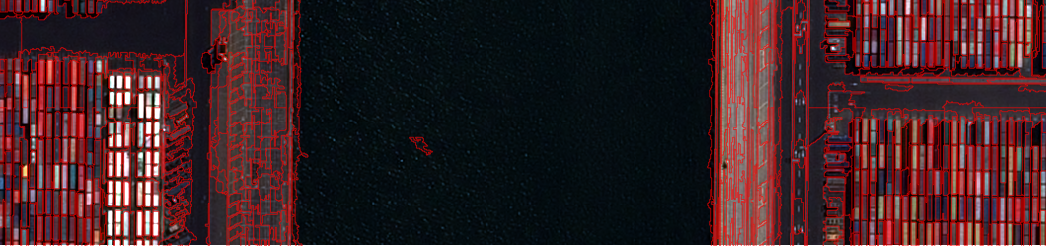
\includegraphics[width=0.45\textwidth]{Pictures/ogrs_stitch_xt.png}}
\caption{Example of large scale segmentation result displayed in QGIS, with stitching}
\end{figure}

The second problem is that the polygons reflect exactly the shape of
the segment, and contain a large amount of vertices. This leads to
very heavy vector files, sometimes even heavier than the corresponding
raster image would be. To deal with this issue, we added
pre-processing as well as post-processing. First, we added an input
mask image to avoid segmenting unwanted regions, like no-data
pixels, clouds, or vegetation (if vegetation is not desired). We also
added a rule to remove very small segments, which are more likely to
correspond to segmentation noise than to real objects (this leads to
holes in the segmentation canvas). Last, we again used the
capabilities of OGR to perform a geometry simplification algorithm,
which simplify polygons by removing vertices according to a given
tolerance.

These additional processing allows to produce a cleaner vector
segmentation output which can then be used in a GIS software.


\section{Examples and figures}

TODO

\section{Conclusion}

  This framework is only a first step toward providing an open source
 large scale OBIA and spatial reasoning framework. Future developments
 will include more stitching and tiling strategies to enhance the
 segmentation performance at tiles borders, and the computation of
 attributes along with polygons, such as statistics on radiometry from
 an image, or shape attributes. These attributes could then be used
 for reasoning or classification at the object level. While there is
 still a lot missing, we hope to provide a comprehensive environment
 for object-based techniques for VHR images analysis through the
 ongoing efforts to integrate Orfeo ToolBox within Quantum
 GIS \cite{}, a open source GIS software, via Sextante \cite{},
 and bridge the gap between remote sensing and GIS.


\subsubsection{References}

\bibliographystyle{acm}
\bibliography{refs}

\end{document}
